\documentclass{report}
\usepackage{graphicx}
\usepackage{hyperref}
\usepackage{adjustbox}
\usepackage{makecell}
\usepackage{boldline}
\usepackage{array}
\usepackage{longtable}
\usepackage{wrapfig}
\usepackage{rotating}
\usepackage{bookmark}

\begin{document}

\title{Project Three Specification}
\author{Connor Byrd, Chad Baxter, Chris Vasquez}
\date{\today}
\maketitle

\renewcommand\thesection{\arabic{section}}
\renewcommand\thesubsection{\thesection.\arabic{subsection}}
\renewcommand\thesubsubsection{\thesubsection.\arabic{subsubsection}}

\section{Introduction}
Provides an overview, explains the document purpose, and how it is organized.\par
\subsection{Document Purpose}
Explain the purpose of this specification document. Make sure that you identify the intended audience for the document.\par
\subsection{System Scope}
Briefly describe the system that you’re building. Provide the motivation for this system. Include a very high level overview (1-2 paragraphs).\par
\subsection{Overview}
Explain how your document is organized. Write a sentence or two summarizing each large section so that if the reader wanted to know where to find some information about the system, they’d have a good idea of where to look within this document.\par
\section{Overall Description}
This section should discuss background information about your system including a definition of client/s, definition of users, and detailed description of the included functionality. This information should be broken into subsections. One example breakdown is shown below.\par
\subsection{Client characteristics}
Who is your client? Why is this system important to him/her/them? This is fictional and can be made-up.\par
\subsection{pkg.User characteristics}
Who are the intended users of the system? Describe them. What characteristics of your users make them unique?  How do users interact with your system?\par
\subsection{Product functions}
Here’s where you should describe the software in more detail than you did in section 1.2 (probably about a page overview plus your use cases). What type of functionality will be included? Describe the features in detail. Document the system functionality with a set of written use case and a system-level use case diagram.\par
\section{System Specification}
Explain your system design. What data will be stored in each class?  What operations will each class include?  What type of relationships will exist between classes in your system? How will the various classes interact? In addition to your text explanations, include a class diagram for your system.\par
\section{Assumptions}
List any assumptions that you have made about the system. You should have a brief introduction statement/paragraph in this section. The actual assumptions should be communicated as a bulleted list.\par


%\section{Diagrams}
%\textit{continued on next page...}
%\clearpage
%
%\begin{sidewaysfigure}[ht]
%  \centering
%    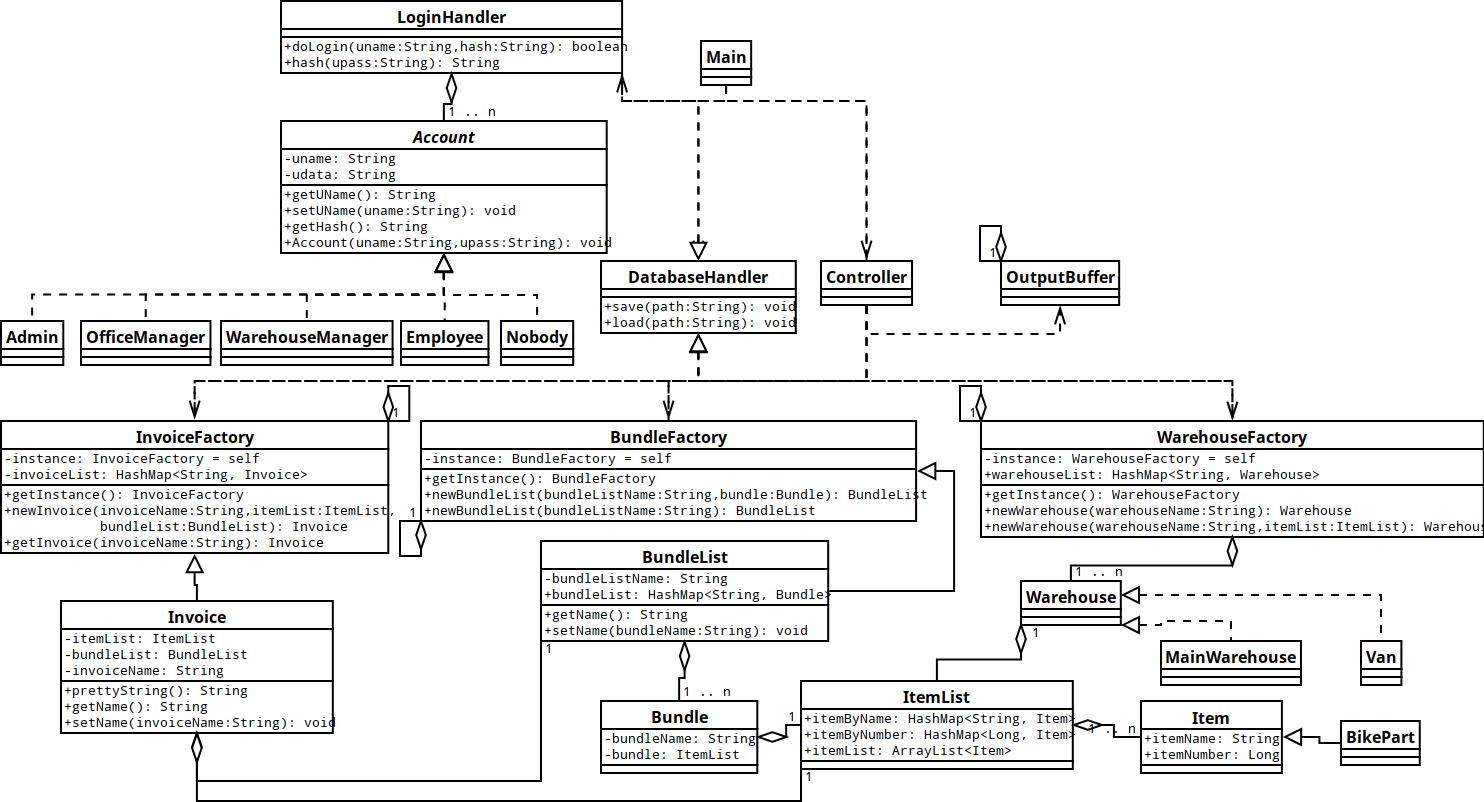
\includegraphics[width=\textwidth,height=\textheight,keepaspectratio]{overview.png}
%  \caption{Class hierarchy.}
%\end{sidewaysfigure}

%\begin{sidewaysfigure}[ht]
%  \centering
%    \includegraphics[scale=0.24,keepaspectratio]{sasequence.png}
%  \caption{Sequence to conduct a sale.}
%\end{sidewaysfigure}

%\begin{figure}[h]
%  \centering
%    \includegraphics[scale=0.5,keepaspectratio]{wmsequence.png}
%  \caption{pkg.Warehouse manager use cases.}
%\end{figure}

%\begin{figure}[h]
%  \centering
%    \includegraphics[scale=0.5,keepaspectratio]{ui.png}
%  \caption{The JavaFX UI for the project.}
%\end{figure}

\end{document}
